% Präambel

% \ für den Befehl {} stehen die wichtigen Argumente und in [] optionale Argumente

% verschiedene Dokumentenklassen: scrartcl, scrreprt, scrbook, beamer
\documentclass[fontsize=11]{scrartcl}

% Pakete laden mit \usepackage[argumente]{paketname}

% Paperränder festlegen
\usepackage[left=15mm, right=15mm, top=25mm, bottom=30mm, paper=a4paper]{geometry}

% für das richtige Encoding
\usepackage[T1]{fontenc}
\usepackage[utf8]{inputenc}

% für die richtige Sprache
\usepackage[german]{babel}

% Paket zur Verlinkung von Dingen
\usepackage{hyperref}

% Paket für Bilder
\usepackage{graphicx}

% Paket was alles etwas schöner macht
\usepackage{lmodern}

% Zitieren
\usepackage[autostyle]{csquotes}
\usepackage[backend=biber,
style=authoryear-icomp]{biblatex}
% Datei mit allen Beschreibungen hinzufügen (ich nutze JabRef zur Erstellung)
\addbibresource{refs.bib}

% Mathematische Pakete
\usepackage{amsmath}
\usepackage{amssymb}
\usepackage{mathtools}

% Für Quellcode
\usepackage{listings}
% Statt Listings wollen wir Quellcode da stehen haben
\renewcommand\lstlistlistingname{Quellcode}
\renewcommand{\lstlistingname}{Quellcode}
\usepackage{pgffor}
% Verschönerungen für Python Code
\usepackage{accsupp}   
\usepackage{xcolor} 
\lstset{
	backgroundcolor=\color{gray!4},  
	basicstyle=\ttfamily\footnotesize,
	breakatwhitespace=false,                     
	captionpos=t,                    
	commentstyle=\color{black!45!green}\itshape, 
	extendedchars=true,              
	frame=single,                   
	keepspaces=true,             
	keywordstyle=\bfseries,                     
	numbers=left,
	stepnumber=1,                
	numbersep=6pt,                   
	numberstyle=\ttfamily\scriptsize\color{black!60}, 
	rulecolor=\color{gray!30},        
	showspaces=false,               
	showtabs=false,  
	showstringspaces=false,                                   
	tabsize=3,                      
	title=\lstname ,
	aboveskip=-0.1cm,
	xleftmargin=2em,
	columns=flexible,
	fontadjust=true, 
	breaklines=true,
	language=python,
	keywordstyle=\bfseries\color{blue!70!black}, % keyword color
	stringstyle=\color{orange} % string color        
}

% Informationen über Author, Titel und Datum
\author{Julien Klaus}
\date{\today}
\title{Kleine Latex Einführung}


% hier startet der Dokumenteninhalt
\begin{document}
	
	% Erzeugen einer Titelseite
	\maketitle
	
	\tableofcontents
	
	% Dokumente können wir in sectionen gliedern
	\section{Abschnitte}
	\subsection{Unterabschnitt}
	\subsection*{Unterabschnitt ohne Nummer}
	\subsubsection{Unterunterabschnitt}
	Weitere Abschnittsbefehle findet man unter
	\url{https://www.namsu.de/Extra/strukturen/Inhaltsverzeichnis.html}.
	
	\section{Textformatierung}
	% Schriftgrößen festlegen
	\tiny klein
	\scriptsize größer
	\footnotesize noch größer
	\normalsize normale Größe
	\large größer als normal
	\LARGE noch größer
	\huge sehr Groß
	\Huge am Größten 
	% wieder zurück zur normal Größe
	\normalsize
	
	% Text auch beliebig formatieren
	\emph{Emphasize}
	\textsf{Serifenfrei}
	\texttt{Monospace}
	\textit{Kursiv}
	\textbf{Fett}
	
	\section{Listen}
	% Listen
	\begin{itemize}
		\item Element A
		\item Element B
	\end{itemize}

	% Aufzählungen
	\begin{enumerate}
		\item Element 1
		\begin{itemize}
			\item Element A 2
			\item Element B 2
		\end{itemize}
		\item Element 2	
	\end{enumerate}

	% Beschreibungsumgebung
	\begin{description}
		\item[Informatik] Macht irgendwas mit Computern
		\item[Mathematik] Macht irgendwas mit Zahlen
	\end{description}

	\section{Bilder}
	Wir können auch beliebige Bilder einfügen.
	\begin{figure}[htb]
		% zentrieren
		\centering
		% Bild laden mit 50% der Textbreite
		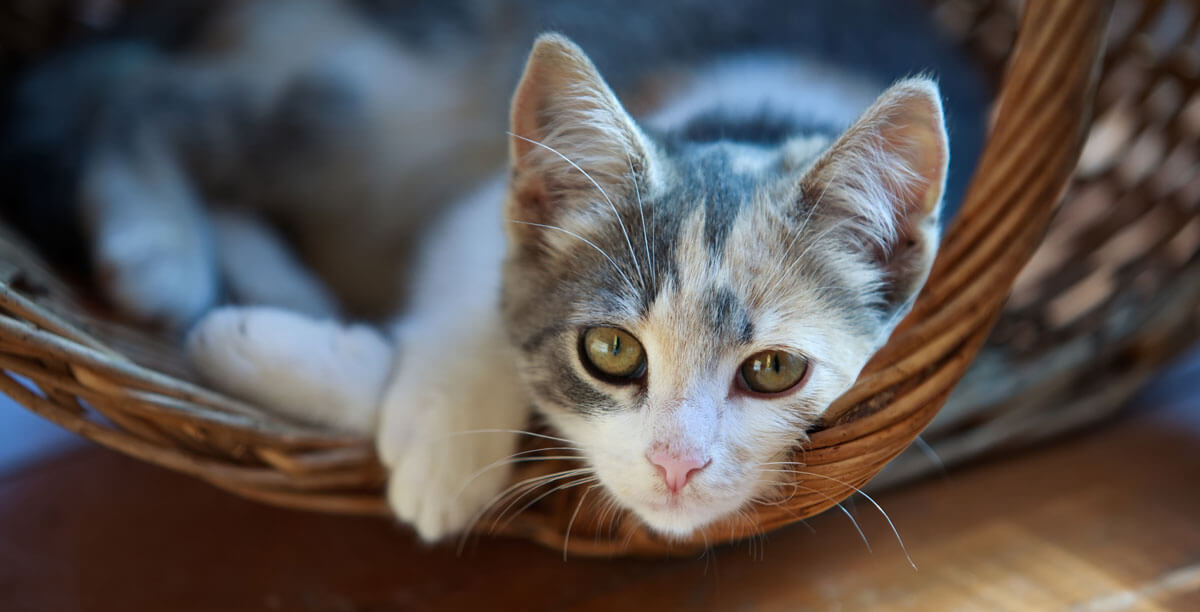
\includegraphics[width=0.5\textwidth]{bild.jpg}
		% Bildunterschrift einfügen
		\caption{Irgendein Bild mit einem Tier}
		% Wir können dem Bild ein Label geben um im Text darauf zu referenzieren
		\label{img:bild}
	\end{figure}
	Im Text kann ich nun auf das Bild \ref{img:bild} verweisen.
	
	\section{Tabellen}
	Tabellen werden in der Umgebung \texttt{table} beschrieben
	\begin{table}[htb]
		% Tabellen bestehen aus Spalten (mit Linien dazwischen)
		\begin{tabular}{l | c r}
			% Linie über der Tabelle
			\hline
			% erste Zeile (beenden mit \\, zwischen den Spalten &
			Index & Beschreibung & Wert \\
			\hline
			\hline
			1 & Wert & 25 \\
			2 & Name & Chlor \\
		\end{tabular}
	\end{table}
	Um schöne Tabellen zu bauen schaut euch doch einfach mal \texttt{prettytable} an.
	
	\section{Mathematik}
	Wir können im Text bliebige Mathematische Dinge angeben $1+2$. Wir hätten auch 1+2 schreiben können. Aber beispielsweise $A\cap B$. Eine Übersicht über verschiedene Mathematische Symbole findet man auf \url{https://de.wikipedia.org/wiki/Liste_mathematischer_Symbole}.
	
	% Für sehr lange Formeln, die außerhalb vom Text stehen. 
	\begin{equation}
		A\cap B = \overline{ (A\cup B)}
	\end{equation}
	
	Wenn wir da keine Nummer haben wollen nutzen wir einen Stern.
	\begin{equation*}
	A\cap B = \overline{ (A\cup B)}
	\end{equation*}
	
	\begin{equation}
		\sum_{\alpha\geq 1}^{\mu \cdot \gamma} = \int_{12}^{45} \frac{\sin{\begin{pmatrix}
		1 & 2 \\
		3 & 4
		\end{pmatrix}}}{A\cap B\leftrightarrow \mu}
	\end{equation}
	
	
	\section{Quelltexte}
	Wir können Quelltext direkt in \LaTeX schreiben oder aus einer Datei laden.
	\lstinputlisting[linerange={1-2}, caption=Etwas Quellcode]{code.py}

	Oder einfach so schreiben. Dann muss der Quelltext allerdings in diesem Dokument sehr weit vorne beginnen.
	\begin{lstlisting}[caption=Genau der gleiche Quellcode]
s = 'pVjisemlr tEmrxfqoqlcgc zikmr nSltzukdnitusm'
print(s[1::2]).
	\end{lstlisting}
	
	
	\section{Zitieren}
	Wir können im Text zitieren zum Beispiel das Latexbuch \cite{Hed09} oder das Mathematikbuch \cite{Tes08}.
	
	
	% Abbildungsverzeichnis
	\listoffigures
	
	\lstlistoflistings
	
	% Literaturverzeichnis
	\printbibliography 
	








	
\end{document}